\section{Métodos de Atenuação de Harmônicas}
%métodos são necessários para mitigar esse problema

Existem métodos bem concebidos na literatura com relação à metodologias para mitigar o problema da utilização de cargas não lineares em sistemas senoidais. Pode-se encontrar, basicamente, três abordagens para eliminar as harmônicas de mais alta frequência, e assim, manter a qualidade de energia dentro de níveis aceitáveis para propiciar segurança operacional de uma aeronave. Tais sistemas serão descritos brevemente a seguir, e a escolha da utilização de filtros ativos em aplicação aeronáutica será melhor elucidada.  

\subsection{Sistemas Passivos}

A caracterização de um sistema passivo dá-se pela ausência de fontes externas de energia para o correto funcionamento de um circuito ou o controle ativo para o mecanismo de comutação ou condicionamento de dispositivos semicondutores, como transistores ou amplificadores operacionais \cite{AN779}. Para essa classe de dispositivos passivos destacam-se os filtros lineares e os retificadores de alto fator de potência sem a presença de comutadores comandados. 

\subsubsection{Filtros Passivos}

Filtros passivos são circuitos dotados de componentes elétricos passivos lineares, como indutores, capacitores e resistores, concebido com objetivo de obter uma função de transferência cujo comportamento típico é atenuar componentes de frequências senoidais específicas. Os filtros são basicamente compostos por impedâncias interligadas e o comportamento destes circuitos depende do valor e da disposição dos elementos lineares envolvidos \cite{Mussoi2004,Kassick2010}. 

Conceitualmente, pode-se considerar a concepção de filtros ideais e reais. De maneira simplificada, os filtros ideais são tais que em determinadas frequências a atenuação é nula e em outras é infinita, ou seja, as amplitudes dos componentes do espectro não se altera em determinadas frequências mas em outras são levadas a zero, respectivamente. Tais filtros não são realizáveis e na pratica são utilizados filtros reais. Esses filtros não possuem uma atenuação infinita, e a diminuição das respectivas amplitudes em função da frequência é dada segundo a ordem do filtro. De maneira geral, a ordem do filtro é dada de acordo com o número de elementos armazenadores de energia concebidos no circuito. Assim, para que o filtro real tenha o mesmo comportamento que o ideal haveria de ter ordem infinita, o que o torna inconcebível. 

Por definição, a frequência de corte ($f_c$) dos filtros reais é definida segundo qual a potência do sinal de saída é tida como a metade da potência do sinal de entrada, ainda, esta definição pode ser estendida como a frequência a qual a razão dos sinais de saída e entrada é tida como $\sqrt{2}$, ou mais, que nessa frequência a atenuação do sinal seja de 3 decibéis.

As principais topologias de filtros passivos podem ser divididos em 4 tipos:

\begin{enumerate}[i),leftmargin=1.75cm,itemindent=0cm] % PODE SER ADULTERADO \begin{enumerate}[i),leftmargin=1.75cm,itemindent=0cm] ou \begin{enumerate}[i),leftmargin=0cm,itemindent=1.75cm]
	\item 
	\textit{Filtro Passa Baixa:} A concepção desse tipo de filtro age de forma a criar caminhos de alta impedância entre a entrada e saída do sistema para frequências mais elevadas que $f_c$ \cite{Kassick2010}. Desse modo, comparativamente ao sinal da entrada, a saída possui a mesma característica de amplitude e potência para frequências menores que $f_c$, mas atenuam componentes do espectro cujo valor é maior que a frequência de corte, ou seja, $f>f_c$. Ainda, deve-se ter em mente que quanto maior o valor da frequência das componentes que compõem o sinal, maior a redução em suas amplitudes \cite{Mussoi2004}. A resposta em módulo do sistema de um filtro passa baixa pode ser visto na figura \ref{fig:LP_filter}.\todo{arrumar esse texo que está porco}

	\item 
	\textit{Filtro Passa Alta:} Analogamente ao filtro passa baixa, os sistemas com a topologia passa alta possuem caminhos de alta impedância para componentes de baixa frequência que são aplicadas na entrada do sistema \cite{Kassick2010}. Desse modo, a saída possui um espectro com a predominância de componentes de alta frequência. Como ocorre nos filtros passa baixa, a frequência que delimita a atenuação é denominada frequência de corte, e componentes com valores mais elevados possuem ganho unitário, ou seja, não são alterados pelo sistema \cite{Mussoi2004}. O espectro típico de um filtro passa alto pode ser visualizado na figura \ref{fig:HP_filter}. 
		
	\item 
	\textit{Filtro Passa Faixa:} Os filtros passa faixa são caracterizados por circuitos cuja resposta apresenta a passagem de sinais com frequências situadas numa faixa intermediária no espectro, atenuando as amplitude dos sinais que estão fora desse intervalo. A frequências que delimitam esta faixa são denominadas frequência de corte inferior ($f_L$) e frequência de corte superior ($f_H$) \cite{Mussoi2004}. Desse modo, o comportamento do sistema caracteriza-se pela atenuação de componentes que possui frequência abaixo de $f_L$ e acima de $f_H$. Outra característica fundamental dos filtros passa faixa é a largura de banda definida pela intervalo onde o sinal não é atenuado. Em termos numéricos, esse valor é definido por $f_H-f_L$. Ainda existe a frequência central $f_0$ ou frequência de ressonância, a qual é a média geométrica entre a frequência de corte inferior $f_L$ e a frequência de corte superior $f_H$ da banda de passagem, ou seja, $f_0=\sqrt{f_L.f_H}$. O módulo da resposta em frequência típica de um filtro passa faixa é mostrada na figura \ref{fig:BP_filter}.
		
	\item 
	\textit{Filtro Rejeita Faixa:} Ao contrário do filtro passa faixa, este tipo de filtro é definido por atenuar componentes cujas frequências estão contidos em um determinado intervalo, enquanto as amplitudes das componentes fora deste não são alteradas.  Analogamente ao passa faixa, existe a frequência de corte inferior e superior definidas por $f_L$ e $f_H$, respectivamente \cite{Mussoi2004}. As componentes com valores de frequência menores que $f_L$ e maiores que $f_H$ são mantidas iguais ao sinal de entrada, ao passo que os componentes contidos dentro do intervalo $f_L\;-\;f_H$ possuem as amplitudes atenuadas. O espectro de frequência desse tipo de filtro pode ser visto na figura \ref{fig:RB_filter}.
		
	\begin{figure*}[!htbp] %Ganho em função da frequência de filtros passivos típicos
		\centering
		\begin{subfigure}[b]{0.48\textwidth}
			\centering
			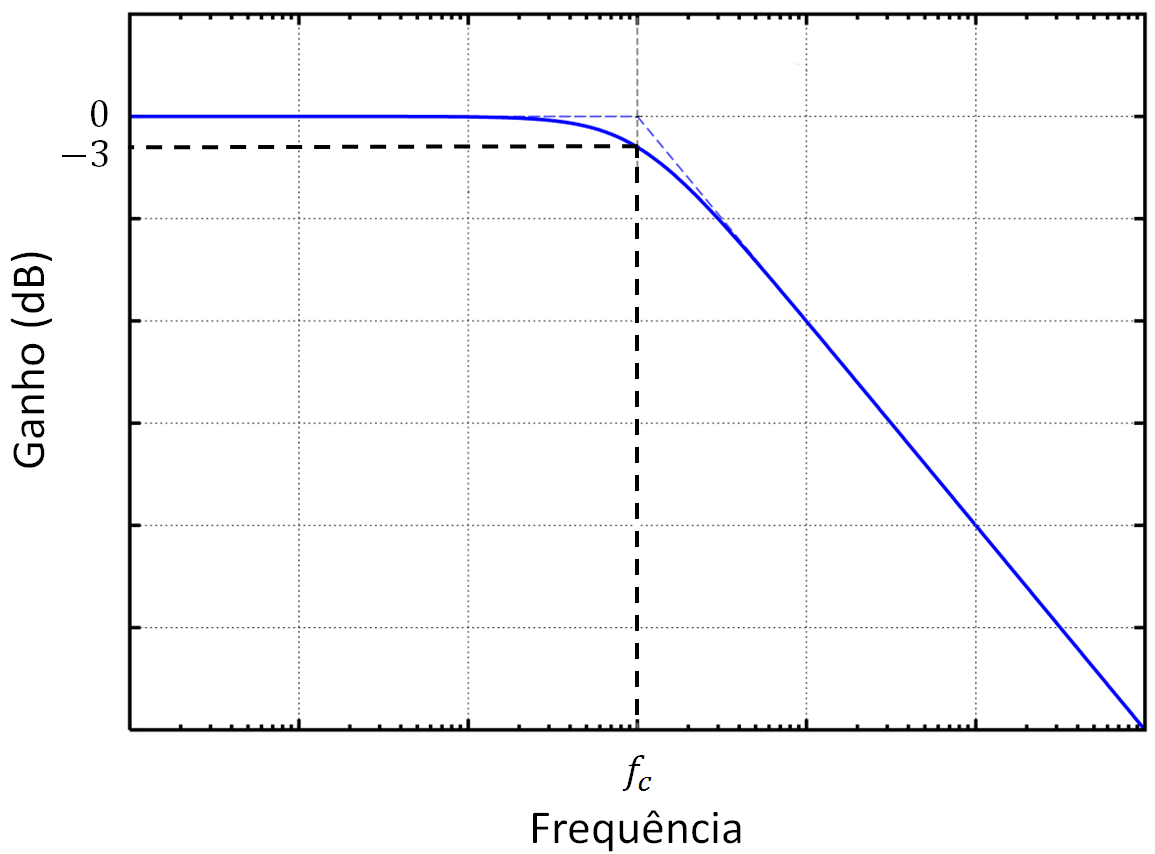
\includegraphics[width=\textwidth]{Cap2/Figuras/LP_filter.png}
			\caption{\centering Resposta em frequência de um filtro passa baixa} 
			\label{fig:LP_filter}
		\end{subfigure}%
		\hfill
		\begin{subfigure}[b]{0.48\textwidth}  
			\centering 
			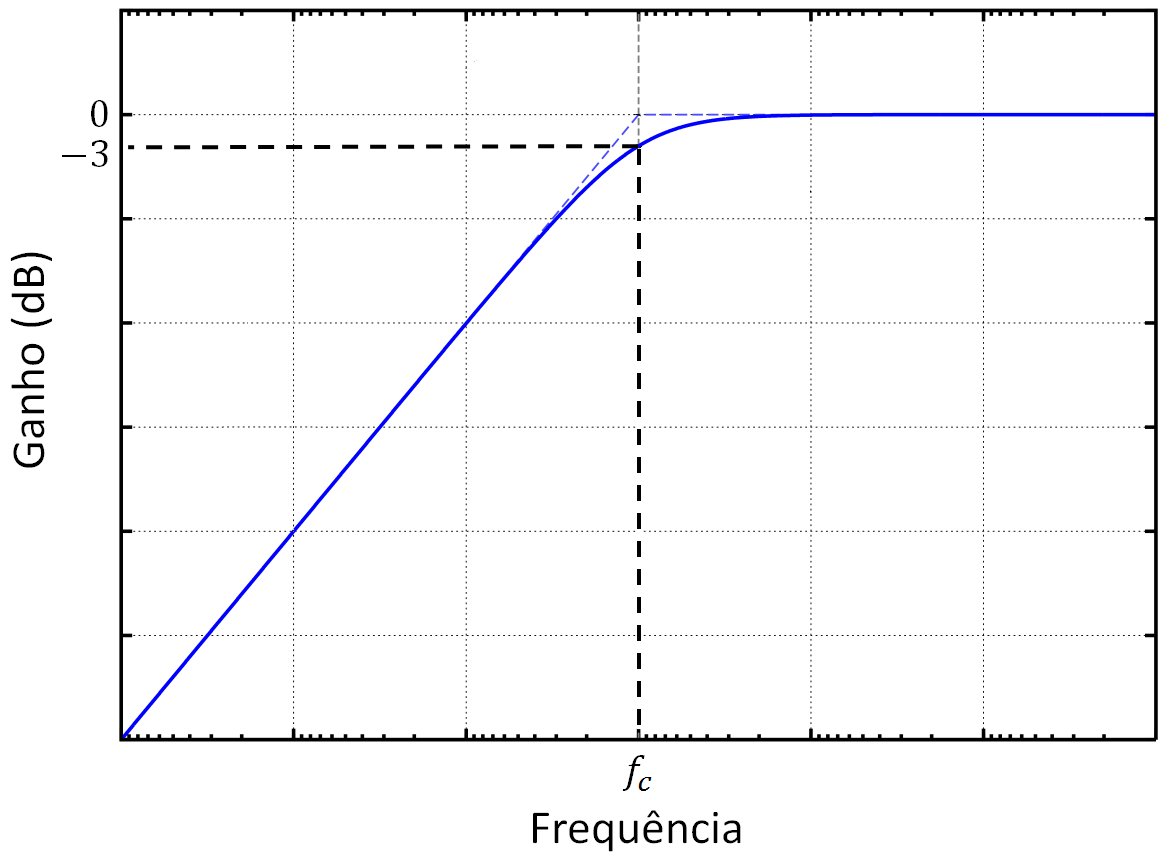
\includegraphics[width=\textwidth]{Cap2/Figuras/HP_filter.png}
			\caption{\centering Resposta em frequência de um filtro passa alta}    
			\label{fig:HP_filter}
		\end{subfigure}%
		\vskip\baselineskip
		\begin{subfigure}[b]{0.48\textwidth}   
			\centering 
			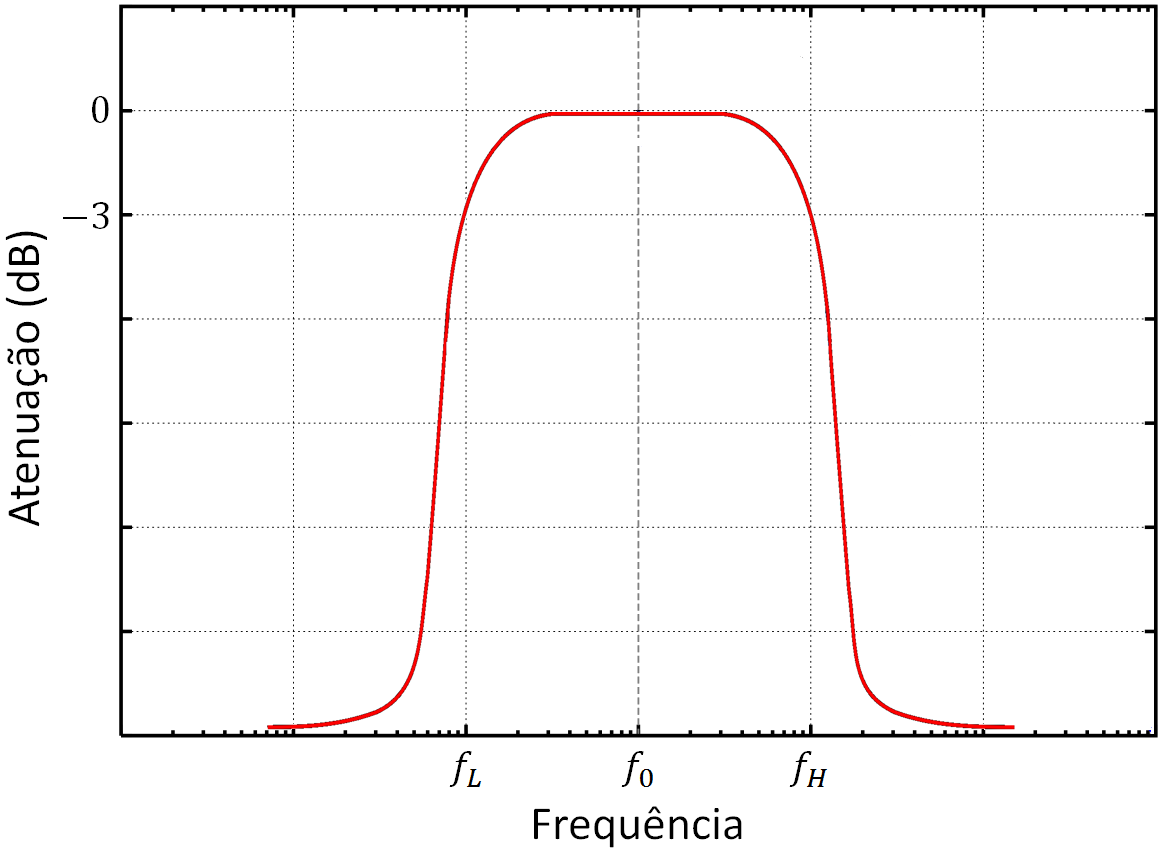
\includegraphics[width=\textwidth]{Cap2/Figuras/BP_filter.png}
			\caption{\centering Resposta em frequência de um filtro passa faixa}   
			\label{fig:BP_filter}
		\end{subfigure}%
		\hfill
		\begin{subfigure}[b]{0.48\textwidth}   
			\centering 
			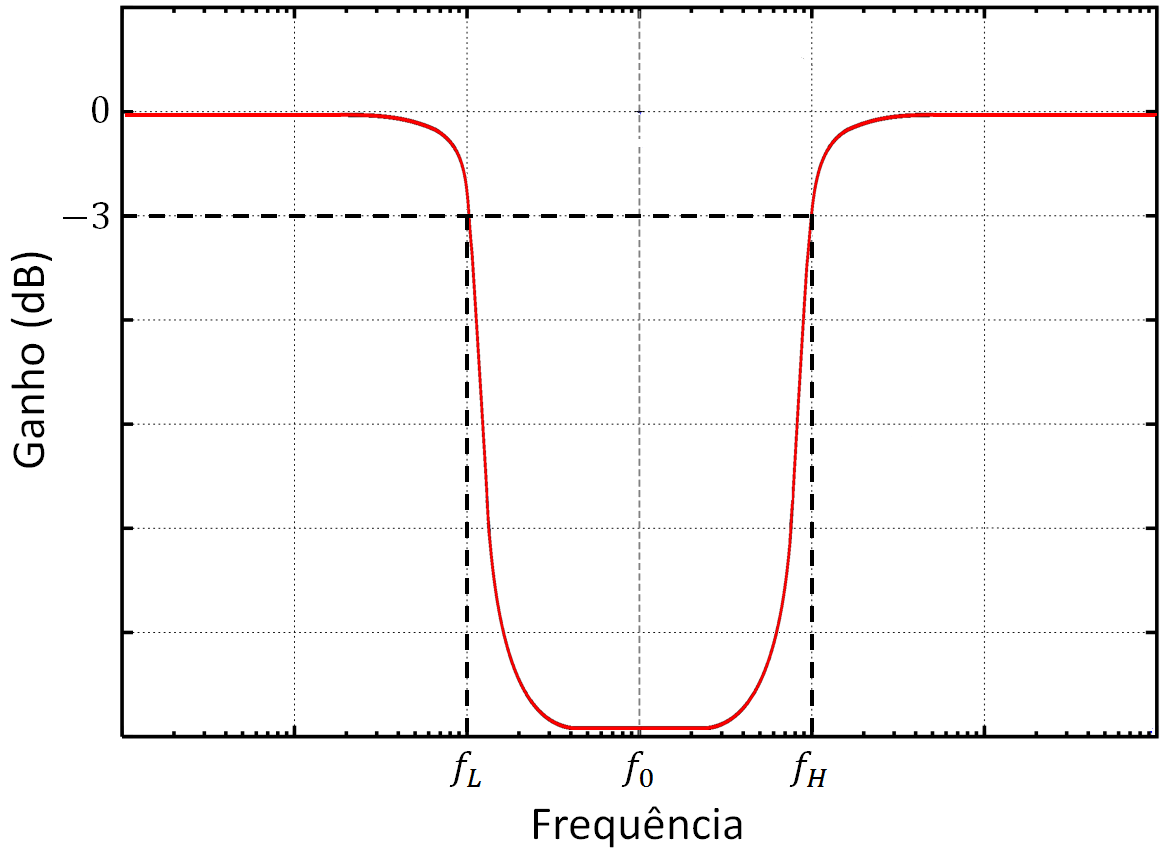
\includegraphics[width=\textwidth]{Cap2/Figuras/RB_filter.png}
			\caption{\centering Resposta em frequência de um filtro rejeita faixa}   
			\label{fig:RB_filter}
		\end{subfigure}%
		\caption{Ganho em função da frequência de filtros passivos típicos} 
		\label{fig:mean and std of nets}
	\end{figure*}
	
\end{enumerate}

Para o problema de atenuar as harmônica de mais alta frequência que a fundamental, a utilização de filtros passa baixa é mais adequada, pois são os componentes harmônicos que acabam por degradar a qualidade de energia do sistema elétrico.

\subsubsection{Retificadores Multipulso}

Neste tipo de circuito o retificador é concebido utilizando uma filosofia semelhante a um retificador comum com pontes de diodo, porém o arranjo dos semicondutores junto com autotransformadores faz com que a corrente requerida da fonte possua uma forma quase senoidal, tornando o retificador com alto fator de potência. Outra particularidade desse conversor é a ausência de controle externo sobre os semicondutores, sendo que os comutadores do retificador realizados por diodos e seu funcionamento depende apenas das tensões e correntes aplicadas sob seus terminais.

Os retificadores são comumente encontrados com as topologias dos circuitos partindo de 12 para arranjos de mais pulsos, como 18, 24, 30 e ainda maiores valores para manter a qualidade de energia  com relação ao \textit{THD} \cite{Singh2008}. No conceito desse retificador existe a montagem com autotransformadores de modo que o arranjo de diodos passam a conduzir de tal forma que a corrente requerida na entrada tenha um formato com baixa incidência de harmônicas de elevada frequência. Ainda, com o aumento de pulsos do conversor aumenta a qualidade de energia, porém eleva a complexidade dos elementos magnéticos do mesmo. Nas figuras \ref{fig:12_pulse} e \ref{fig:18_pulse} são mostrados típicos retificadores de 12 e 18 pulsos, respectivamente, com suas específicas formas de onda. Aqui fica evidente a melhora na forma da corrente senoidal do retificador de 18 pulsos com relação ao de 12 \cite{Singh2008}.

\begin{figure*}[!htbp] %Circuito típico de um retificador de 12 pulsos com sua respectiva corrente de entrada
	\centering
	\begin{subfigure}[b]{0.49\textwidth}
		\centering
		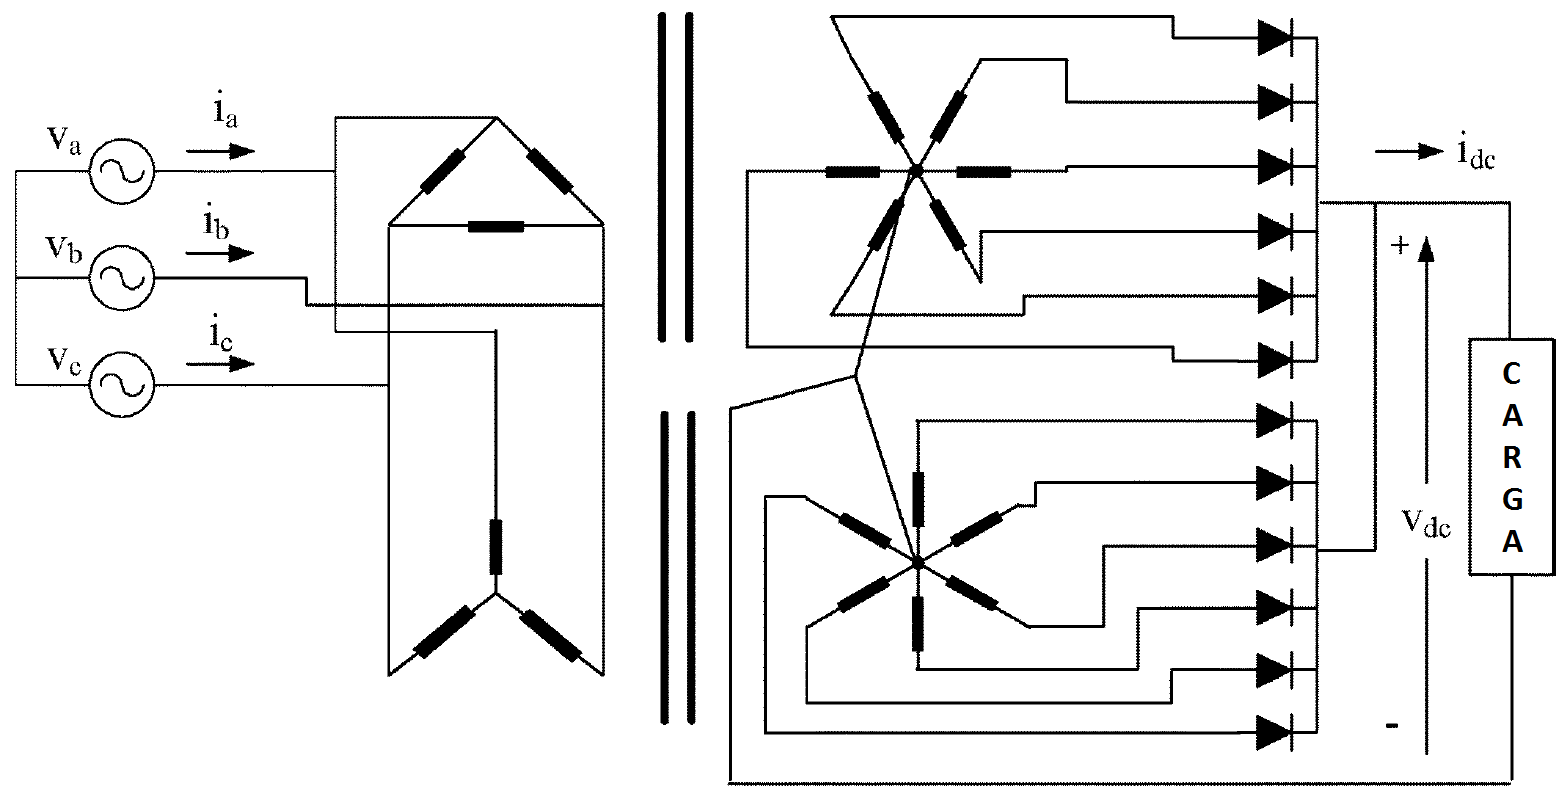
\includegraphics[width=\textwidth]{Cap2/Figuras/12_pulse_rectifier.png}
		\caption{Circuito do retificador de 12 pulsos} 
		\label{fig:12_pulse_rectifier}
	\end{subfigure}%
	\hfill
	\begin{subfigure}[b]{0.49\textwidth}  
		\centering 
		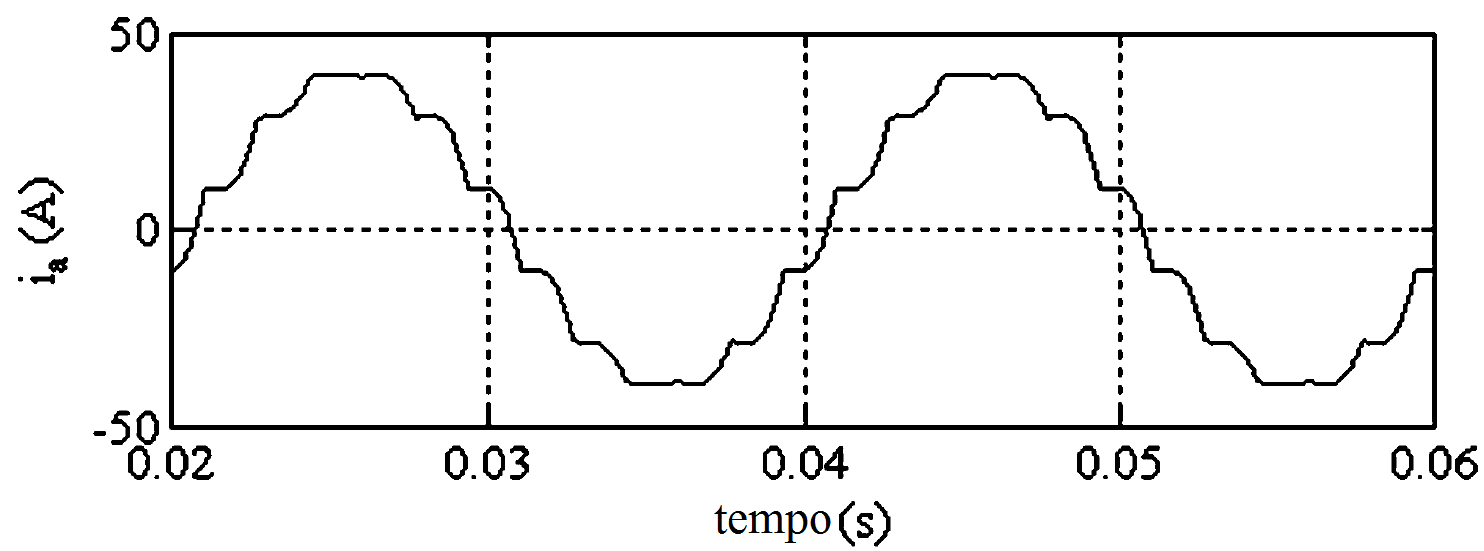
\includegraphics[width=\textwidth]{Cap2/Figuras/12_pulse_wave.png}
		\caption{Forma de onda da corrente de entrada}    
		\label{fig:12_pulse_wave}
	\end{subfigure}%
	\caption{Circuito típico de um retificador de 12 pulsos com sua respectiva corrente de entrada \cite{Singh2008}}
	\label{fig:12_pulse}
\end{figure*}

\begin{figure*}[!htbp] %Circuito típico de um retificador de 18 pulsos com sua respectiva corrente de entrada
	\centering
	\begin{subfigure}[b]{0.49\textwidth}
		\centering
		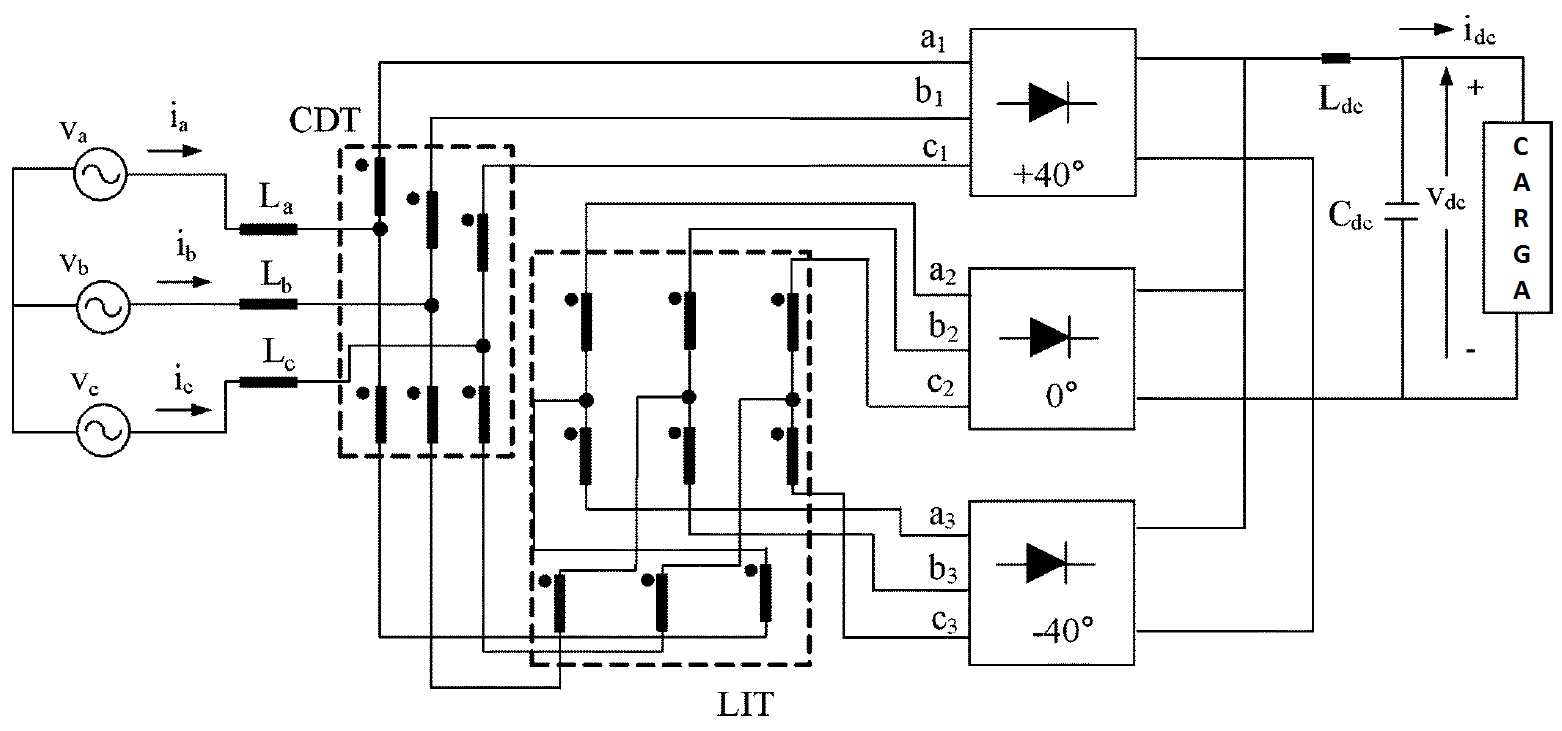
\includegraphics[width=\textwidth]{Cap2/Figuras/18_pulse_rectifier.png}
		\caption{Circuito do retificador de 18 pulsos} 
		\label{fig:18_pulse_rectifier}
	\end{subfigure}%
	\hfill
	\begin{subfigure}[b]{0.49\textwidth}  
		\centering 
		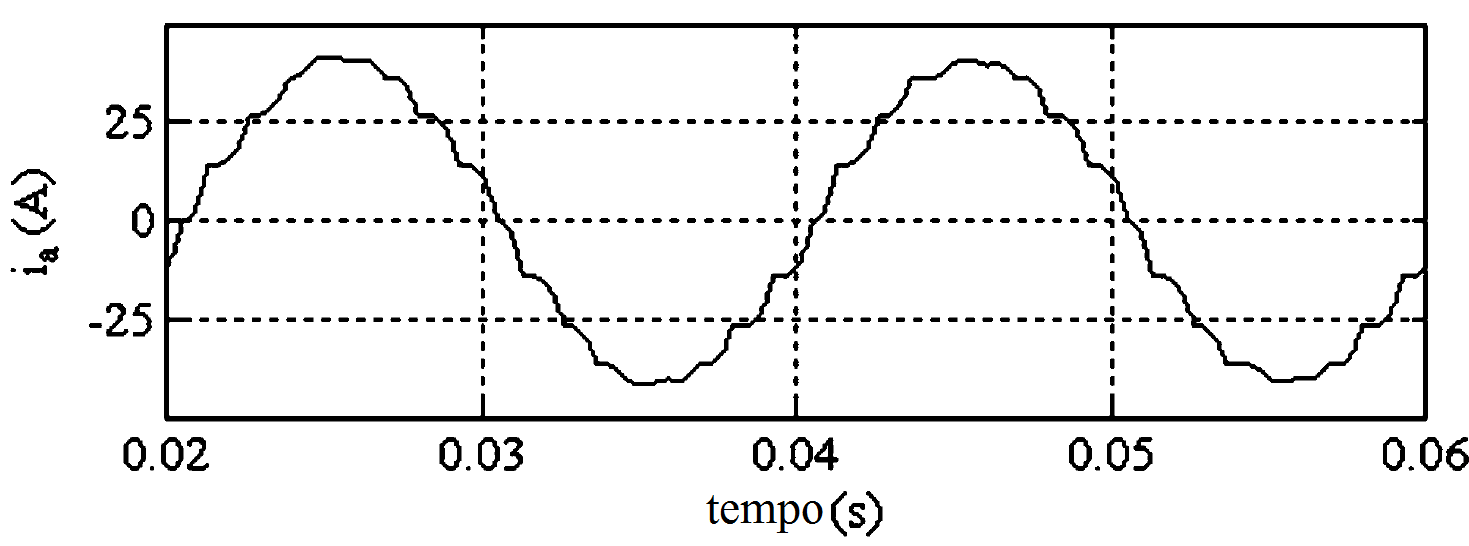
\includegraphics[width=\textwidth]{Cap2/Figuras/18_pulse_wave.png}
		\caption{Forma de onda da corrente de entrada}    
		\label{fig:18_pulse_wave}
	\end{subfigure}%
	\caption{Circuito típico de um retificador de 18 pulsos com sua respectiva corrente de entrada \cite{Singh2008}}
	\label{fig:18_pulse}
\end{figure*}

Cabe lembrar que a utilização de retificadores multipulso é realizável tanto em redes de 60 Hz quanto em sistemas de elevada frequência, tal qual 400-800 Hz \cite{Gong2003,Lobo2005}. Isto faz-se necessário para atender o mercado aeronáutico que possui o sistema elétrico operando em 400 Hz, ou até 800 Hz para geração em frequência variável.

\subsection{Sistemas Ativos}

Em sistemas ativos os conversores são operados com a implementação de chaves estáticas com comutação controlada cujo objetivo é diversificar as topologias e, dentro de certas faixas de operação, reduzir as perdas por condução quando comparados com circuitos comutados por diodos. Com isso, a flexibilidade de projeto é aumentada de modo que há uma maior diversificação de tipos de retificadores disponíveis. Além do mais, com o comando na comutação é possível haver uma melhor regulação da tensão na saída do sistema e, utilizando certas topologias, um controle de corrente de entrada de modo a proporcionar um fator de potência em acordo com os requisitos de qualidade de energia do sistema.

Dois dos principais tipos de sistemas ativos implementados para mitigar as harmônicas do sistemas são os conversores de alto fator de potência e os filtros ativos. No primeiro caso os retificadores têm seus componentes ordenados de forma que o controle na comutação dos semicondutores proporcionam 

Outra forma de atenuação de componentes harmônicas no sistema é a utilização de inversores controlados conectados na entrada de uma carga com baixo fator de potência de de maneira a filtra ativamente as componentes de alta freqüência. 

O controle da intensidade da tensão/corrente na saída desse tipo de conversor pode ser utilizado para injetar corrente no sistema de modo a anular os harmônicos presentes no sistema.

\subsubsection{Conversores com Correção de Fator de Potência}

\subsubsection{Filtros Ativos}

\section{Vantagens e Desvantagens dos Sistemas de }\todo{Melhorar o título visto que alguns métodos não atenuam e sim ja implementam a solução com alto fator de potência}

\begin{figure}[!htbp]
	\centering
	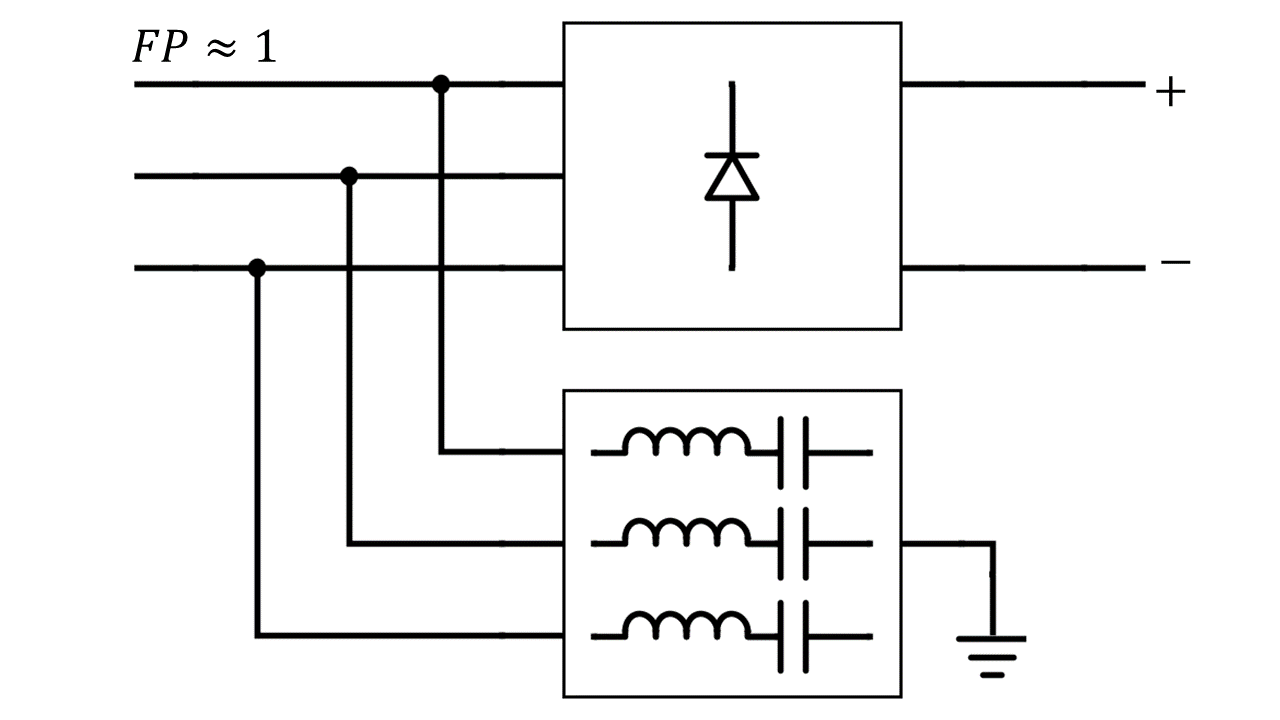
\includegraphics[width=0.65\textwidth]{Cap2/Figuras/sch_filtro_passivo.png}
	\caption{Filtro Passivo}
	\label{fig:sch_filtro_passivo}
\end{figure}

\begin{figure}[!htbp]
	\centering
	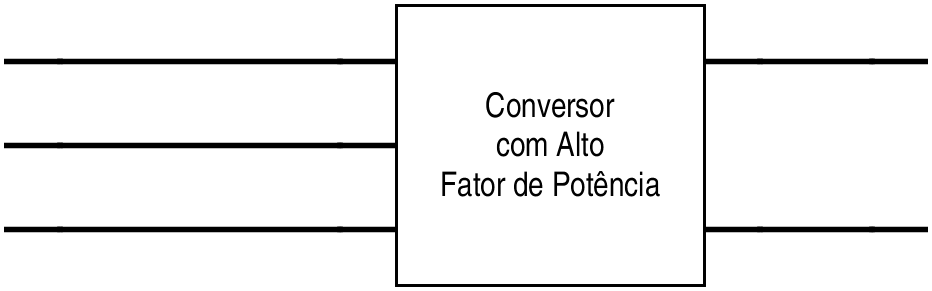
\includegraphics[width=0.65\textwidth]{Cap2/Figuras/sch_PFC.png}
	\caption{Filtro PFC}
	\label{fig:sch_PFC}
\end{figure}

\begin{figure}[!htbp]
	\centering
	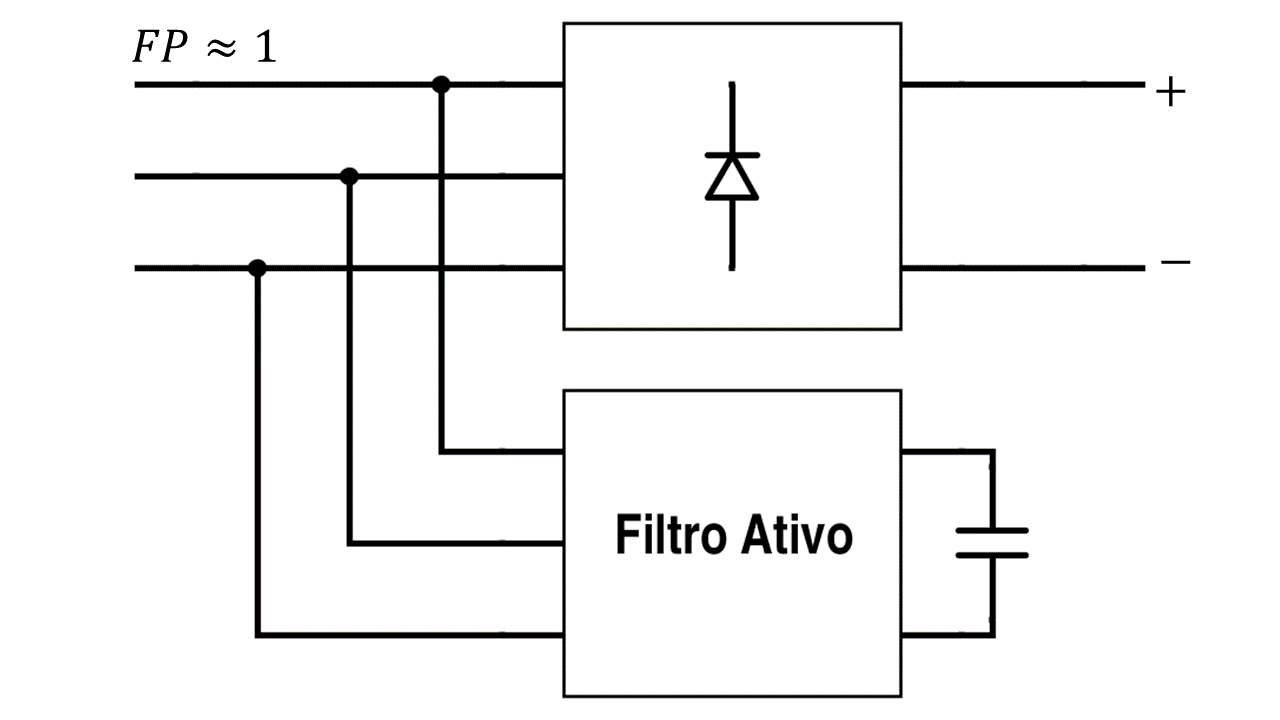
\includegraphics[width=0.65\textwidth]{Cap2/Figuras/sch_filtro_ativo.png}
	\caption{Filtro Ativo}
	\label{fig:sch_filtro_ativo}
\end{figure}



